% -*- mode: latex; mode: auto-fill; coding: utf-8; -*-

\label{sec:finite_element_method}
% downwards rewritten from page 3-5
The \defit{finite element method} (FEM) is a numerical analysis tool
used for calculating approximate solutions and is employed to find
solutions to a wide variety of different engineering and physics
problems.
%
The method, which is diverse and flexible, can be applied to complex
problems where analytical solutions seldom exist or are too "expensive"
to solve. As this is precisely the case with many problems in the broad
field of continuum mechanics, where the complex shape of a continuum
needs to be approximated, the method is used extensively within this
field.
%
The finite element method envisions the continuum body or
\defit{solution region} as an assembly of many small,
interconnected subregions (elements), the same way continuum mechanics
does.
In the finite element method the size and number of the elements are
finite in contrast to continuum theory, where the subregions are
considered infinitesimal.
A \defit{finite element model} of a given problem is a
piecewise approximation to the continuum body. That is: The basic
premise of the finite element method is that the \defit{solution
  region} can be approximated by an assemblage of discrete finite
elements. Because the elements can have different shapes and can be
assembled in a many ways, they can be used to approximate exceedingly
complex geometrical shapes \citebook{page~3-5}{book:fem-engineers}.
% upwards rewritten from page 3-5

\section{Basic Concepts and Fundamentals}
% downwards: rewritten from fem-engineers, p. 5-6
When dealing with a continuum problem in any dimension the
\defit{field variable} or \defit{nodal variable} is the unknown value
that we are trying to find. Examples of field variables include:
pressure, temperature, displacement, etc. and they can be either
scalars, vectors, or higher-order tensors.
%
Field variables capture infinitely many values because they are a
continuous function over the continuum body.
Therefore the problem has an infinite number of unknowns.
%\emph{
The finite element discretization reduces the
problem to one with a finite number of unknowns, this is done by
dividing the continuum body into elements and expressing the
unknown field variable in terms of approximation functions within each
element.
%}
The \defit{approximation functions}, also called \defit{shape functions},
\defit{basis functions}, or \defit{interpolation functions}, are
defined in terms of the field variable value at specified
points in the body called \defit{nodes} or \defit{nodal points}.
Nodes are usually located where adjacent elements are connected
(\defit{element boundaries}). In addition to the nodes located on the
element boundaries, the element may also have other nodes. 
We distinguish between two different kinds of nodes: Nodes are called
\defit{exterior nodes} if they lie on the element boundary and
\defit{interior nodes} otherwise. 
To completely define the behaviour of the field variable within an
element, the nodal values of the field variable and the interpolation
functions for the element are used.
%\emph{
But because we want to find this field variable the nodal values of
the field variables become the unknowns.
%}
Once we have found the unknowns, the interpolation functions define
the field variable continuously throughout all elements.
%
Clearly the precision of the approximation depends both on the size
and number of elements and on the interpolation functions.
As one would expect, we cannot choose the interpolation functions
arbitrarily, certain \defit{compatibility conditions} must be
satisfied. Often the functions are chosen so the field
variables or their derivatives are continuous across adjoining element
boundaries hereby meeting the compatibility conditions, which is
exactly what we will do.
%
The most important feature of the finite element method, which
distinguishes it from other numerical methods, is its ability to
formulate solutions for individual elements before assembling these to
represent the entire problem.
This means that if we are analysing a problem like, for example, the
one in chapter \vref{sec:framework_for_equilibrium_problems} relating
external forces to elongation of the
springs, we first concentrate on modeling the problem for a single
element, and then assemble these to model the entire problem. In
essence, a complex problem is reduced to a series of greatly
simplified ones. \citebook{page~5-6}{book:fem-engineers}.
% upwards: rewritten from fem-engineers, p. 5-6

\section{Constructing and Solving the Model}
\label{sec:using-the-FEM}
% downwards: rewritten from fem-engineers, p. 7
Solving a continuum problem via the finite element method
always follows an orderly step-by-step procedure. In general this procedure
can be summarized into a list of steps one must perform to construct
and evaluate a problem. This list is shown below.
% upwards: rewritten from fem-engineers, p. 7
In the following subsections, each of the steps will be carefully
explained and in chapter \vref{sec:applying-fem}, we will go through
how our model has been constructed using the same stepwise approach
\citebook{page~7-8}{book:fem-engineers}.


\begin{itemize}
\item Discretize the solution region
\item Select interpolation function
\item Find element properties
\item Assemble the element properties to obtain the system equations
\item Impose boundary conditions
\item Solve the system equations
\item Make additional computations
\end{itemize}

Note that some of these steps, like "Find element properties" and
"Assemble the Element properties to obtain the system equation"
essentially covers the same thing as the equilibrium framework discussed
in chapter \vref{sec:framework_for_equilibrium_problems}. In this
section we use a more structured approach for constructing and solving
the system. Furthermore: We will adapt a more abstract view of what an
element is and describe in detail how the interpolation functions
work.

\section{Discretize the Solution Region} % (page 7 FEM book)
\label{sec:discretize-the-continuum}
% downwards: rewritten from fem-engineers, p. 7-8
Because the finite element method envisions the solution region as
built up of many small elements the first step is to divide this
region into elements.
% upwards: rewritten from fem-engineers, p. 7-8
%
% downwards rewritten from page 86-87, generalising elements + piecewise
In chapter \vref{sec:framework_for_equilibrium_problems}, when
we considered the equilibrium framework,
our idea of what an element is was directly linked to physical
phenomena of the problem.
%
We imagined the elements to be individual segments or parts of the
actual system, that is: A physical thing as for example a spring has a
one to one correspondence to an element.
%
In this case the nodes belonging to an element were part of the element
itself and because the unknown field variable was displacement the
nodes could move as the element deformed.
%
%We now generalize the definition of an element.
We want to think of elements in less physical terms and instead use a
more mathematical interpretation of the concept.
%
So instead of viewing an element as a physical part of the system, we
think of it as a part of the solution domain. We imagine the
solution domain as being divided into subregions sectioned by lines or
planes. If the solution domain has curved boundaries, the curves are
approximated by a series of straight line or flat plane segments. These
lines or planes define the boundaries between elements and the
elements are only interconnected at imaginary node points on the
boundaries. In this way the solution domain is discretized into
a patchwork of elements, as illustrated in figure \vref{fig:patchwork}
for a two-dimensional body.
%
% \{For problems where displacement is the unknown field variable we no
% longer need to imagine that the elements deform or change shape.
% Instead we define a displacement field (in terms of the interpolation
% functions) in the regions of space where the elements are located.
% The element nodes are then simply locations in space where the
% displacement are known or sought. All this will be elaborated later when
% the interpolation functions have been introduced.}

\begin{figure}
  \centering
  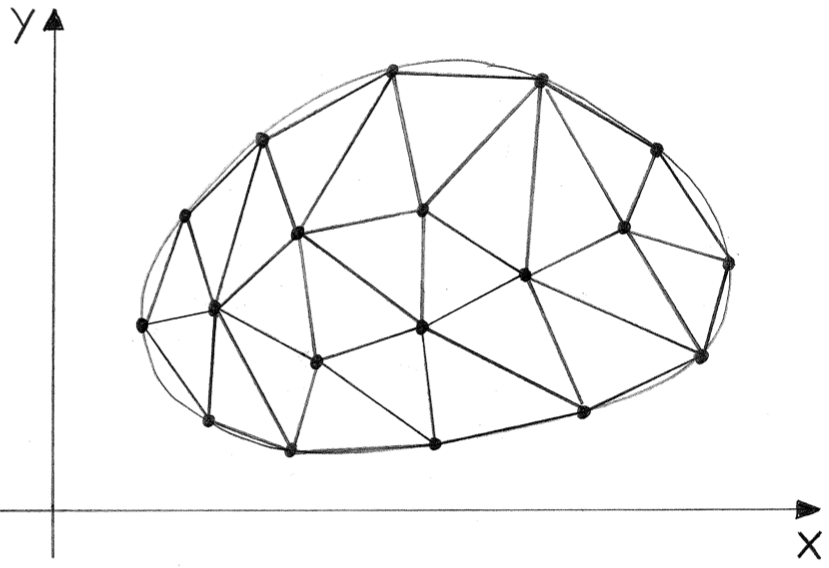
\includegraphics[width=8cm]{./images/finite_element_method_patchwork.png}
\caption{A discretized two-dimensional solution domain.}
\label{fig:patchwork}
\end{figure}

Mathematically a finite element mesh is interpreted as a spatial
subdivision \citebook{page~86-87}{book:fem-engineers}.
% upwards rewritten from page 86-87, generalising elements + piecewise
%
In one dimension the element covers a distance, in two the element
covers an area and in three dimensions it is a volume.
%
Depending on the number of spatial dimensions of the solution domain
the elements have different characteristics. In one-dimensional space
the most common element has two nodes which are connected by a
line. This element type is called a bar, a truss or a beam
element and is illustrated in figure \vref{fig:2line}.
%
So the simplest element in two dimensions, one that covers an area, is
the three-node triangular element and in three dimensions the four-node
tetrahedron as shown in figure \ref{fig:3triangle} and figure
\vref{fig:4tetrahedron}, respectively.
%
The element types are denoted by how many nodal points they have.
Note that the number of nodes has nothing to do with the element's
geometrical shape, but is chosen because of other considerations (e.g.
type of interpolation functions).

\begin{figure}
  \centering
  \subfloat[Two-node line element.]{
    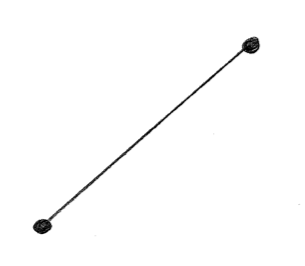
\includegraphics[width=3cm]{./images/finite_element_method_line.png}
    \label{fig:2line}
  }
  \hspace{10mm}
  \subfloat[Three-node triangle element.]{
    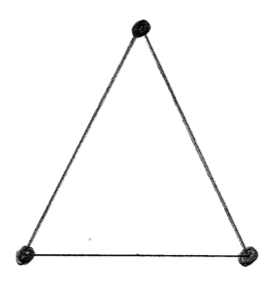
\includegraphics[width=2.8cm]{./images/finite_element_method_triangle_3nodes.png}
    \label{fig:3triangle}
  }
  \hspace{10mm}
  \subfloat[Four-node tetrahedral element.]{
    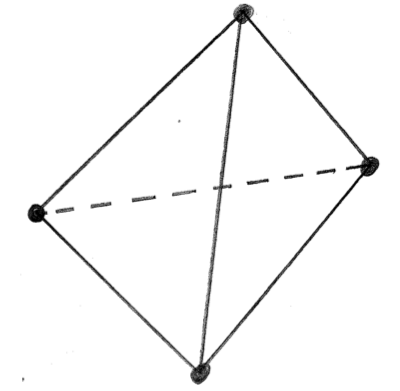
\includegraphics[width=3cm]{./images/finite_element_method_tetrahedron_4nodes.png}
    \label{fig:4tetrahedron}
  }
  \caption{Simplest element types in one, two, and three dimensions.}
  \label{fig:simple-elements}
\end{figure}

When considering more than one dimension the range of different
element types to choose from becomes larger.
%In two-dimensional space there is a wide range of different element
%types to choose from.
To get an idea of the range we show various kinds of
two-dimensional elements with different shape and number of
nodes. Figure \vref{fig:2d-elements}
illustrates quadratic elements and figure
\vref{fig:triangle-element-family} triangular elements.

\begin{figure}
  \centering
  \subfloat[Four-node rectangle element.]{
    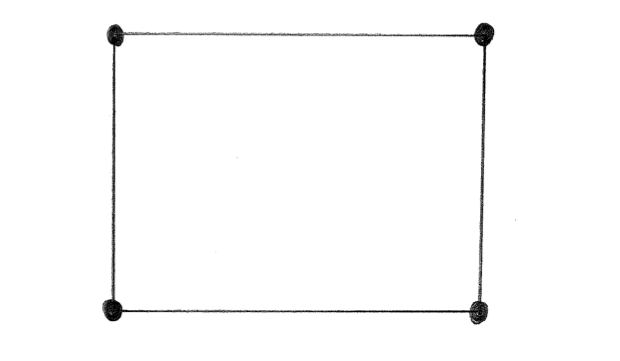
\includegraphics[width=4cm]{./images/finite_element_method_rectangle_4nodes.png}
    \label{fig:4rectangle}
  }
  \hspace{10mm}
  \subfloat[Four-node quadrilateral element.]{
    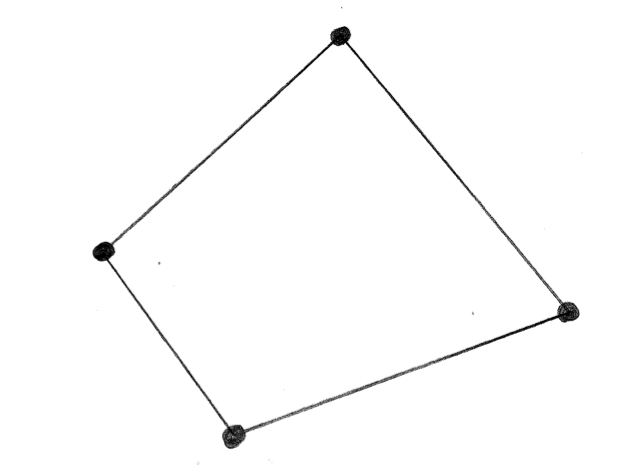
\includegraphics[width=4cm]{./images/finite_element_method_quad_4nodes.png}
    \label{fig:4quadrilateral}
  }
  \caption{Examples of two-dimensional elements.}
  \label{fig:2d-elements}
\end{figure}

% downwards rewritten from 144, degrees of freedom
In addition to the shape, two other features characterizes a
particular element type:

\begin{itemize}
\item The number of nodes assigned to the element
\item The number and type of nodal variables chosen for it.
\end{itemize}

The number and type of nodal variables assigned to an element are
called the element's \defit{degree of freedom} (DOF). If for example we have a
three-node element, where a two-dimensional displacement vector are
the nodal variable, then the element have six degrees of freedom. The
degrees of freedom for an element is the same as the number of
independent variables \citebook{page~144}{book:fem-engineers}.
% upwards rewritten from 144, degrees of freedom

\begin{figure}
  \centering
  \subfloat[Three-node triangle element.]{
    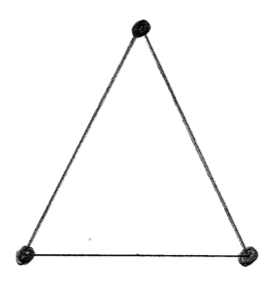
\includegraphics[width=3cm]{./images/finite_element_method_triangle_3nodes.png}
    \label{fig:2nd3triangle}
  }
  \hspace{10mm}
  \subfloat[Six-node triangle element.]{
    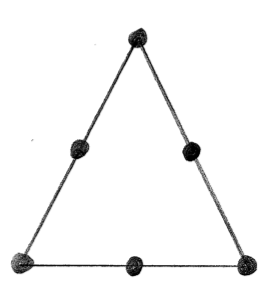
\includegraphics[width=3cm]{./images/finite_element_method_triangle_6nodes.png}
    \label{fig:6triangle}
  }
  \hspace{10mm}
  \subfloat[Ten-node triangle element.]{
    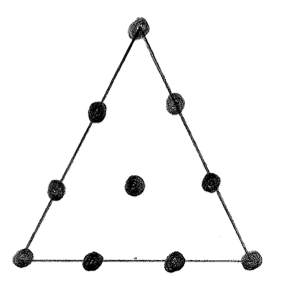
\includegraphics[width=3cm]{./images/finite_element_method_triangle_10nodes.png}
    \label{fig:10triangle}
  }
  \caption{Examples of members from the triangular element family.}
  \label{fig:triangle-element-family}
\end{figure}

Element types with the same shape but with different number of nodes
are called an \defit{element family}. An example of members from the
triangular family is the three-node, six-node and ten-node triangular
elements as shown in figure \ref{fig:2nd3triangle},
\ref{fig:6triangle}, and \vref{fig:10triangle} respectively. Note that
the ten-node triangular element is an example of an element with one
interior node. \\

By increasing the number of nodes in an element, the degrees of
freedom increases hereby facilitating more complex interpolation
functions. The nodal variables can be use
to express non-linear interpolation functions. Consider using a
two-node line element as the element type. The line with its two nodes
have two nodal variables which can express a first order polynomial
equal to a linear interpolation:

\begin{equation*}
P(x) = ax + b
\end{equation*}

if we increase the number of nodes in the element by inserting an
extra node at the midpoint of the line we get three nodal variables
and can now use a second order polynomial to express a non-linear
interpolation: 

\begin{equation*}
P(x) = ax^2 +bx + c
\end{equation*}

As the number of element nodes increases so does the order of the
polynomial we use as the interpolation
function. Higher order interpolation functions gives more control over
how the interpolation functions act inside an element. But the
interpolation functions must have convergence at the element
boundaries hereby satisfying the compatibility conditions, and
although we choose a higher order polynomial the interpolation
functions are only continuous across element boundaries but not
differentiable.
%
The consequences of using a higher order interpolation function with
more nodes at each element is that the per element calculations get
more complex and more time consuming. Instead of increasing the
number of nodes for each element it is also an option to increase
the number of elements, hereby approximating complex
interpolation functions with more elements. Whether to choose fever
elements and high order interpolation functions or more elements
is up for discussion. Higher order polynomials as
interpolation functions are further discussed in
\citebook{page~144-146}{book:fem-engineers}.
We chose the simplest of the two, that is we stick to
$1^{st}$ order polynomials for each element in a high resolution mesh.\\


% \{
% Advanced knowledge:
% Selecting an element type can be broken into two choices. First the
% element shape is chosen, then the number of nodes we use to model the
% element. The shape can be chosen without considering the interpolation
% functions, but the number of nodes is chosen to fit whatever
% interpolation functions we want to use.
% Interpolation functions are mostly chosen to be polynomials.
% Polynomials have orders and can be define in n dimensions.
% The dimensions for the polynomial is determined by the type of element
% that has been chosen. That is the element and the interpolation
% functions should have the same dimensions, so for example, if the
% element is two-dimensional then so is the polynomial. The order of the
% polynomial however is linked the number of nodes we chose to represent the
% element. That is, the number of nodes in the element most be equal to the
% number of coefficients in the polynomial.
% %
% For the triangular family illustrated in figure
% \vref{fig:triangle-element-family}, the three-node
% triangle is used together with a $1^{st}$ order polynomial, the six-node
% triangle with a $2^{nd}$ order, and the ten-node triangle is used
% together with a $3^{rd}$ order polynomial. This is because a $1^{st}$
% order polynomial in two dimensions have three coefficients, a $2^{nd}$
% have six, and a $3^{rd}$ order have ten coefficients.
% %
% Higher order interpolation functions gives more control over
% how the interpolation functions acts inside an element. But the
% interpolation functions most have convergence at the element
% boundaries, and although we chose a higher order polynomial the
% interpolation functions at the boundaries continues to be linear.
% %
% The consequences of using a higher order interpolation functions with
% more nodes at each element is that the per element calculations gets
% more complex and more time consuming.
% %
% Here religion enters the discussion. Instead some argues the it is
% better the use less complicated per element calculations and higher
% mesh resolution.
% %
% To the best of our knowledge this discussion has not been
% settled, and no data for or against either sides has been provided.
% %
% Therefore we chose the simplest of the two, that is we stick to
% simple calculations per element and a high resolution mesh
% %
% \citebook{page~144-146}{book:fem-engineers}.
% }

In three-dimensional space the range of element types
becomes even larger and mixed with the fact that element boundaries
can be curved, called ISO-parametric elements, this gives endless
possibilities for combinations. In figure \vref{fig:3d-elements} some
examples of three-dimensional elements are shown.

\begin{figure}
  \centering
  \subfloat[Prism.]{
    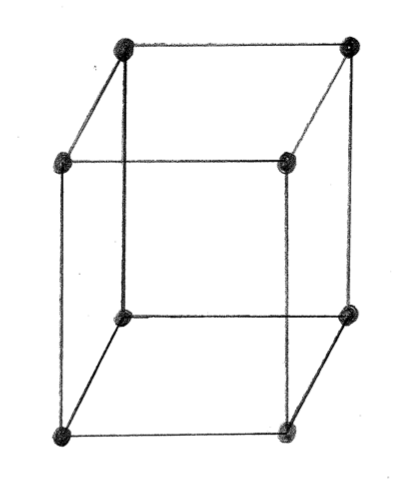
\includegraphics[width=3cm]{./images/finite_element_method_right_prism_8nodes.png}
    \label{fig:8general-prism}
  }
  \subfloat[General hexahedron.]{
    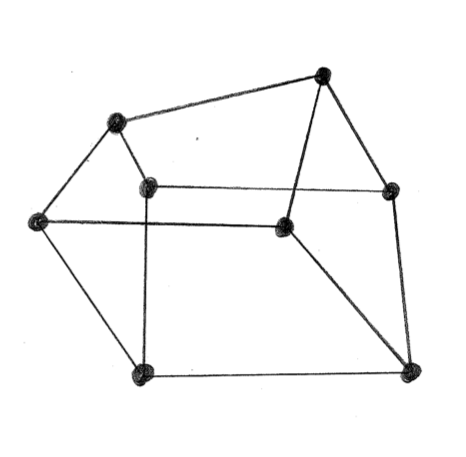
\includegraphics[width=4cm]{./images/finite_element_method_hexahedron_8nodes.png}
    \label{fig:8general-hexahedron}
  }
  \subfloat[ISO-parametric hexahedron.]{
    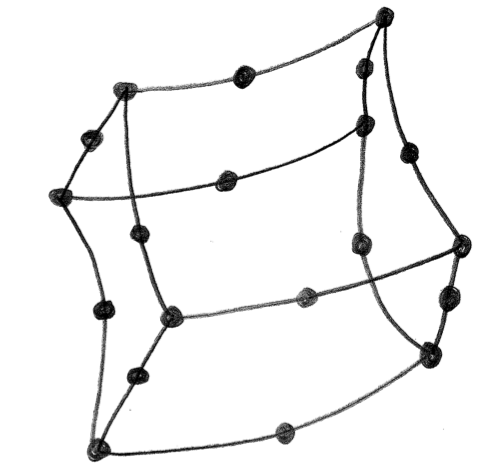
\includegraphics[width=4cm]{./images/finite_element_method_iso_hexahedron_8nodes.png}
    \label{fig:8isoparametric-hexadron}
  }
  \caption{Examples of three-dimensional elements.}
  \label{fig:3d-elements}
\end{figure}

When assembling the elements to cover the solution region, different
shape and mixed types of elements may be used. As this further
increases the complexity of the governing equations we will stick to
one element type.

\subsection{Element and Node Numbering}
The elements share nodes therefore the logistics of keeping track of which
nodes belong to a specific element and in which order the nodes should
be used becomes a challenge. To keep track of this the common thing to do
is to make a table containing the information. This table is called an
\defit{element table} an it relates \defit{element numbers} and
\defit{local node numbers} to \defit{global node numbers}. As this is
best illustrated through an example, figure \vref{fig:node-numbering}
shows a domain discretized into triangular elements, and table
\vref{table:element-table} the associated element table
\citebook{page~15-16}{notes:danish-oil}.

\begin{figure}
  \centering
  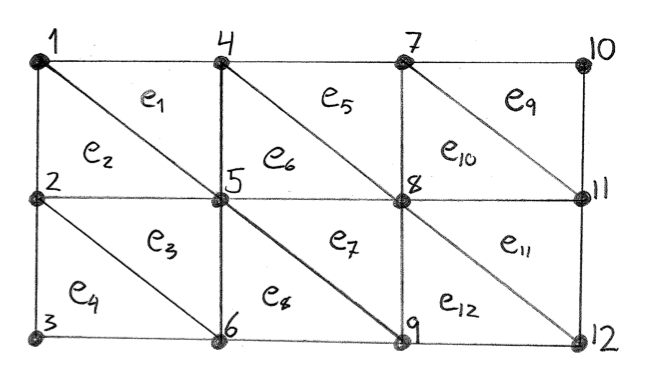
\includegraphics[width=8cm]{./images/finite_element_method_node_numbering.png}
\caption{Global and local node numbering of domain discretized into
  triangular elements.}
\label{fig:node-numbering}
\end{figure}

\begin{table}
  \centering
\begin{tabular}{c|c|c|c|}
n & 1 & 2 & 3 \\
\hline
$e_1$ & 4 & 1 & 5 \\
$e_2$ & 2 & 5 & 1 \\
\vdots & \vdots & \vdots & \vdots \\
$e_{12}$ & 9 & 12 & 8 \\
\hline
\end{tabular}
\caption{Example of an element table.}
\label{table:element-table}
\end{table}

The table indexes the elements by the number $n$ of element $e_n$
in the left column, and local node numbers 1, 2, and 3 in the top
row. The table is then filled with the global node numbers for each
element. An example element ($e_2$) is shown in figure
\vref{fig:node-numbering}, where local node number 2 corresponds to the
global node number 5. 

\section{Selecting the Interpolation Functions}
% downwards: rewritten from fem-engineers, p. 7-8
\label{sec:selecting_interpolation_function}
The next step is to choose the interpolation functions. The
interpolation functions represent the field variable and its
variation over an element. Polynomials are often selected as
interpolation functions because they are easy to integrate and
differentiate.
% upwards: rewritten from fem-engineers, p. 7-8
%
The interpolation functions, make it possible to describe the field
variable continuously over the volume of the element. That is, they
describe the field variable at any given point within or at the
boundary of the element.
%
The collection of interpolation functions for the entire solution
domain provides a piecewise approximation to the field variable.

% downwards: rewritten from fem-engineers, p. 87-90
\subsection{Example of a Piecewise Approximation}
\label{sec:piecewise-approximation}
To illustrate this piecewise approximation we consider
an example of a two-dimensional field variable $\phi(x,y)$.
We will illustrate how $\phi$'s nodal values uniquely and continuously
define $\phi(x,y)$ for the entire solution domain in the $x$-$y$
plane. At the same time, we will introduce the notation used for the
interpolation functions.
%To illustrate the piecewise approximation we focus on a particular
%problem and its solution domain.
Suppose that we have a problem with the solution domain as shown in figure
\vref{fig:patchwork}. This domain has
been sectioned into
three-node triangular elements with exterior nodes at the vertices of
the triangles connecting the elements.
%
This type of domain discretization allows us to select $\phi$ to vary
linearly over an element. The linear variation can be
illustrated as in figure
\vref{fig:piecewise-functions-over-triangle}.

% fem-engineers figure 3.3
\begin{figure}
  \centering
  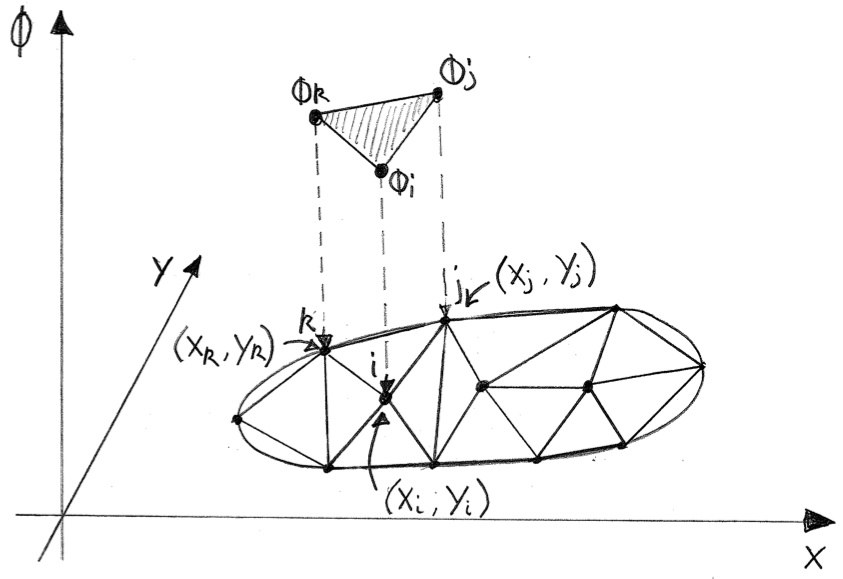
\includegraphics[width=10cm]{./images/finite_element_method_piecewise_functions_over_triangle.png}
\caption{Subdivided domain and piecewise linear solution surface.}
\label{fig:piecewise-functions-over-triangle}
\end{figure}

The first step in finding
the interpolation functions is to mathematically describe the plane passing
through the three nodal values of $\phi$ associated with element
$e$. This is done in equation \eqref{eq:phi}.

\begin{equation}
\label{eq:phi}
\phi^{(e)}(x,y) = \beta_1^{(e)} + \beta_2^{(e)} x + \beta_3^{(e)} y
\end{equation}

Equation \eqref{eq:phi} can then be rewritten to express the constants
$\beta_1^{(e)}$, $\beta_2^{(e)}$, and $\beta_3^{(e)}$ in terms of the
global Cartesian coordinates at the element nodes and the nodal values
of $\phi$. The rewriting is done by evaluating equation \eqref{eq:phi}
at each node, which results in equation \eqref{eq:4phi}.

\begin{equation}
\label{eq:4phi}
\begin{aligned}
\phi_i^{(e)} &= \beta_1^{(e)} + \beta_2^{(e)} x_i + \beta_3^{(e)} y_i \\
\phi_j^{(e)} &= \beta_1^{(e)} + \beta_2^{(e)} x_j + \beta_3^{(e)} y_j \\
\phi_k^{(e)} &= \beta_1^{(e)} + \beta_2^{(e)} x_k + \beta_3^{(e)} y_k
\end{aligned}
\end{equation}

\layoutnewpage

Separating the $\beta_i$'s gives:

\begin{equation}
\label{eq:4beta}
\begin{aligned}
\beta_1^{(e)} &= \frac{ \phi_i(x_j y_k - x_k y_j) + \phi_j(x_k y_i -
  x_i y_k) + \phi_k(x_i y_j - x_j y_i)}{2 \Delta} \\
\beta_2^{(e)} &= \frac{\phi_i(y_j - y_k) + \phi_j(y_k - y_i) +
  \phi_k(y_i - y_j)}{2 \Delta} \\
\beta_3^{(e)} &= \frac{\phi_i(x_k - x_j) + \phi_j(x_i - x_k) +
  \phi_k(x_j - x_i)}{2 \Delta}
\end{aligned}
\end{equation}

where

\begin{equation}
\label{eq:2area-triangle}
2 \Delta = 
\begin{vmatrix}
1 & x_i & y_i \\
1 & x_j & y_j \\
1 & x_k & y_k
\end{vmatrix}
= 2
\begin{bmatrix}
\mbox{area of triangle with} \\
\mbox{vertices $i,j,k$}
\end{bmatrix}
\end{equation}

and by substituting equation \eqref{eq:4beta} into equation
\eqref{eq:phi} and rearranging its terms, we get

\begin{equation}
\label{eq:phi-functions}
\phi^{(e)}(x,y) =
\frac{a_i + b_i x + c_i y}{2 \Delta} \phi_i +
\frac{a_j + b_j x + c_j y}{2 \Delta} \phi_j +
\frac{a_k + b_k x + c_k y}{2 \Delta} \phi_k
\end{equation}

where

\begin{equation}
a_i = x_j y_k - x_k y_i \qquad
b_i = y_j - y_k \qquad
c_i = x_k - x_j
\end{equation}

the other coefficients are obtained through cyclic permutation of
the subscripts $i$, $j$, and $k$. If i=1, j=2, and k=3, the
coefficients are given explicitly by equation \eqref{eq:2d-all-terms}

\begin{equation}
\label{eq:2d-all-terms}
\begin{aligned}
a_1 = x_2 y_3 - x_3 y_2 \qquad b_1 = y_2 - y_3 \qquad c_1 = x_3 - x_2 \\
a_2 = x_3 y_1 - x_1 y_3 \qquad b_2 = y_3 - y_1 \qquad c_2 = x_1 - x_3 \\
a_3 = x_1 y_2 - x_2 y_1 \qquad b_3 = y_1 - y_2 \qquad c_3 = x_2 - x_1
\end{aligned}
\end{equation}

For each element $e$ we now define

\begin{equation}
N_n^{(e)} = \frac{a_n + b_n x + c_n y}{2 \Delta} \quad n=i,j,k
\end{equation}

and let

\begin{equation}
\phi^{(e)} =
\begin{Bmatrix}
\phi_i \\ \phi_j \\ \phi_k
\end{Bmatrix}
\qquad
N^{(e)} = 
\begin{bmatrix}
  N_i^{(e)} & N_j^{(e)} & N_k^{(e)}
\end{bmatrix}
\end{equation}

where $\phi^{(e)}$ is a column vector, $N^{(e)}$ is a row vector.
The functions $N^{(e)}$ are exactly the functions known as the
interpolation functions. In matrix notation we write equation
\eqref{eq:phi-functions} as

\begin{equation}
\label{eq:phi-and-N-functions}
\phi^{(e)}(x,y) = N^{(e)} \phi^{(e)} =
N_i \phi_i + N_j \phi_j + N_k \phi_k
\end{equation}


If the domain has been discretized into $M$ elements, the equations
for the field variable over the entire domain is given by

\begin{equation}
\label{eq:system-phi-functions}
\phi(x,y) = \sum_{e=1}^M \phi^{(e)}(x,y) = \sum_{e=1}^M N^{(e)} \phi^{(e)} 
\end{equation}

We see from equation \eqref{eq:system-phi-functions} that if we know
the nodal values of $\phi$, then we can represent the complete
solution surface $\phi(x,y)$ as a series of interconnected triangles.
The resulting many-faced surface has no gaps between elements and no
discontinuities because the values of $\phi$ at any boundary uniquely
determines the linear variation of $\phi$ along the two nodes defining
that boundary.
%
Although we used a particular interpolation function and a particular
element type
%, that is linear interpolation functions and three-node triangle elements
to obtain equation \eqref{eq:phi-and-N-functions} and
\eqref{eq:system-phi-functions}, these equations are general.
%
When using other element types and more complex interpolation
functions the form of the equations remains the same, it is only the
number of terms in the rows and columns of the matrices that differs.
This means that we can represent the unknown field variable in each element
as in equation \eqref{eq:system-eq-matrixform} if a solution domain is
subdivided into elements \citebook{page~87-90}{book:fem-engineers}.

\begin{equation}
\label{eq:system-eq-matrixform}
\phi = N^{(e)} \phi^{(e)}
\end{equation}

% upwards: rewritten from fem-engineers, p. 87-90

% downwards: rewritten from fem-engineers, p. 37
\subsection{Global and Local Coordinates}
Regardless of how we find the element properties, it is more
convenient and easier to derive the matrix equations for the element
properties in a coordinate system associated with the element (a local
coordinate system). This is exactly the approach we followed for
triangular elements above. Because the local coordinate system, in this
case, is a function of the geometry and orientation of the element,
the local coordinate system for each element may differ.
%
When local coordinate systems are used, it becomes necessary to
transform the element matrices to the common global coordinate system
before the individual element matrices are assembled into the system
equations. This must be done to preserve all element characteristics
in relation to the other elements. Converting between two different
coordinate systems is called \defit{coordinate transformation} and 
is required when the nodal unknowns are components of a vector
\citebook{page~37}{book:fem-engineers}.
Note that displacements are typical field variables where the nodal
unknowns are vectors, so we must be careful to insure that
coordinate transformation occur. When we assemble the element
properties, in section \vref{sec:finding-the-element-properties}, we
will see that the coordinate transformations are part of each
element's stiffness matrix. Because of this the transformations are done
for each element before the whole system is considered.

% upwards: rewritten from fem-engineers, p. 37

% downwards: rewritten from fem-engineers, p. 151-157
\subsection{Natural Coordinates}
The definition of a local coordinate system relies on the element
geometry and all coordinates (described in that
local coordinate system) range between zero and unity, then the
coordinate system is known as a \defit{natural coordinate system}.
A natural coordinate system has the property that when describing a
point located precisely on one of the element's nodes, then one of the
local coordinates of the point have unite value (the coordinate
corresponding to this particular node), and the value zero in all
its other local coordinates.
Between nodes the values of the coordinates vary, but they
always sum to unity. Natural coordinate
systems can be constructed for a variety of elements including:
two-node line element, three-node triangular elements,
four-node quadrilateral elements, four-node tetrahedral
elements and so on.
%
% found on: http://en.wikipedia.org/wiki/Barycentric_coordinates_%28mathematics%29
Natural coordinates for a simplex (a triangle, a tetrahedron, etc.) are
also called \defit{barycentric coordinates}.
%
A particularly advantageous benefit of natural coordinates is that:
When we use these coordinates to derive the interpolation functions,
then integration can be done in a special closed form making it easier
to evaluate the integrals in element equations.
%
Natural coordinates basically describe the location of any point
inside an element in terms of that element's exterior nodes. The
local natural coordinates within an element are denoted by: $L_i$
where $i \in \{1, 2, ..., n\}$ and $n$ is the number of external nodes
of the element. There is always one coordinate associated with a node
$i$ that has unit value in this particular node.
%
By going through some examples it will become clear that local natural
coordinates are functions of the global Cartesian coordinate system
\citebook{page~151-157}{book:fem-engineers}.

\subsection{Natural Coordinates in One Dimension}
To define a natural coordinate system for a two-node line
element, we select $L_1$ and $L_2$ as the natural
coordinates. Then a point $x$ can be expressed as a linear
combination of the nodal coordinates $x_1$ and $x_2$, as follows:

\begin{equation}
\label{eq:1d-linear-combination}
x = L_1 x_1 + L_2 x_2
\end{equation}

We may interpret the coordinates $L_1$ and $L_2$ as weighting
functions relating the coordinates at the end nodes to the coordinate
of any point inside the element. Furthermore these weighting functions
cannot be independent, since they must obey

\begin{equation}
\label{eq:1d-sum-to-one}
L_1 + L_2 = 1
\end{equation}

If we solve equation \eqref{eq:1d-linear-combination} and
\eqref{eq:1d-sum-to-one} simultaneously the result is the functions
$L_1$ and $L_2$, as follows:

\begin{equation}
L_1(x) = \frac{x_2 - x}{x_2 - x_1} \qquad L_2(x) = \frac{x - x_1}{x_2 - x_1}
\end{equation}

The functions $L_1$ and $L_2$ should be interpreted as simply being
the ratio of lengths and are therefore also called \defit{length
  coordinates}. The variation of $L_1$ and $L_2$ within a single
element is illustrated in figure \vref{fig:graph-of-length-coords}.

% fem-engineers figure 5.12
\begin{figure}
  \centering
  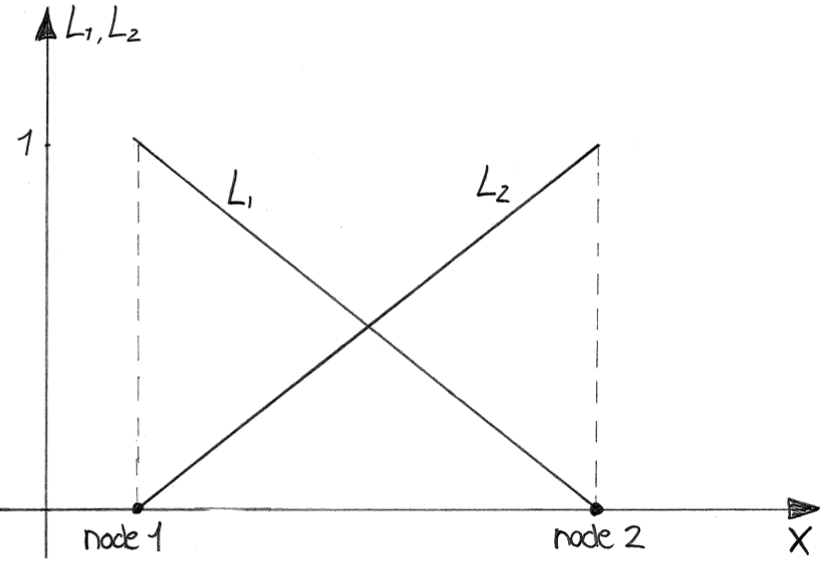
\includegraphics[width=8cm]{./images/finite_element_method_graph_of_length_coords.png}
\caption{Variation of length coordinated within a line element.}
\label{fig:graph-of-length-coords}
\end{figure}

Hence the linear combination of a field variable $\phi$ can be written as

\begin{equation}
\phi(x) = \phi_1 L_1 + \phi_2 L_2
\end{equation}

\subsection{Natural Coordinates in Two Dimensions}
Developing natural coordinates for the three-node triangular element
uses the same approach as in the one-dimensional
case. Again, the goal of the procedure is to find the coordinates
$L_1$, $L_2$, and $L_3$ that describe the location of any point $x$
within the element or on its boundary. The point $(x,y)$ is illustrated
inside a triangular element in figure \vref{fig:point-in-triangle}.

% fem-engineers figure 5.13
\begin{figure}
  \centering
  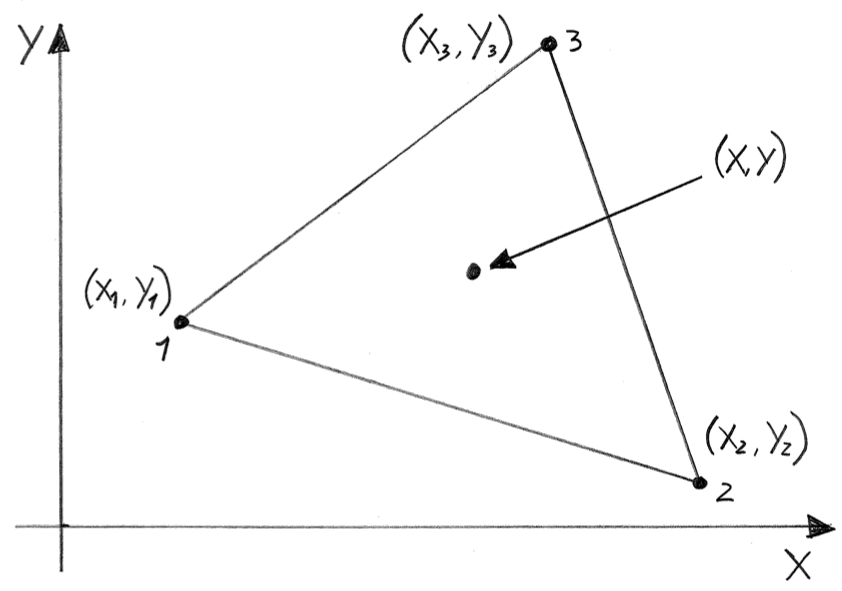
\includegraphics[width=8cm]{./images/finite_element_method_point_in_triangle.png}
\caption{Triangular element with point ($x$,$y$).}
\label{fig:point-in-triangle}
\end{figure}

The relationship between the global Cartesian coordinates of the point
$(x,y)$ within the element, and the new local natural coordinates, that we
are constructing, should have a linear dependence. The linear property
holds for the following equations

\begin{equation}
\begin{aligned}
\label{eq:2d-linear-combination}
x =& L_1 x_1 + L_2 x_2 + L_3 x_3 \\
y =& L_1 y_1 + L_2 y_2 + L_3 y_3
\end{aligned}
\end{equation}

In addition to the equation above, requiring linear dependence, we
again require that the weighting functions sum to unity:

\begin{equation}
\label{eq:2d-sum-to-one}
L_1 + L_2 + L_3 = 1
\end{equation}

It is clear, from equation \eqref{eq:2d-sum-to-one}, that only two of
the natural coordinates can be independent. Intuitively this must be
the case, because if we describe any point as a linear combination of
two points in the global coordinate system (two of an element's nodal
points in global space), then there are only two independent
coordinates if the described point lies inside the element.
When solving  equations \eqref{eq:2d-linear-combination} and
\eqref{eq:2d-sum-to-one} simultaneously for $L_1$, $L_2$, and $L_3$ as
done in equation \eqref{eq:local-coordinates-of-triangle}, the result
gives the natural coordinates in terms of the global coordinates.

\begin{equation}
\label{eq:local-coordinates-of-triangle}
\begin{aligned}
L_1 (x,y) =& \frac{1}{2 \Delta} (a_1 + b_1 x + c_1 y) \\
L_2 (x,y) =& \frac{1}{2 \Delta} (a_2 + b_2 x + c_2 y) \\
L_3 (x,y) =& \frac{1}{2 \Delta} (a_3 + b_3 x + c_3 y)
\end{aligned}
\end{equation}

Where $2 \Delta$ is given by equation \eqref{eq:2area-triangle} on
page \pageref{eq:2area-triangle}.
%
Recalling the linear piecewise approximation example from section
\vref{sec:piecewise-approximation}, we conclude that the natural coordinates
$L_1$, $L_2$, and $L_3$ are identical to the linear interpolation
functions. This means that: $N_i = L_i$ for the
three-node triangular element when using a linear interpolation function.
The natural coordinates for a triangle have an analogous
interpretation to length coordinates. For both the line element and
the triangular element $L_i$ is a ratio, in the case of the line it
describes the ratios of lengths, but for the triangle it is a ratio
of areas. Figure \vref{fig:area-coords} illustrates how the natural
coordinates for the triangular element, often called
\defit{area coordinates}, are related to areas. When a point is
located on the boundary of the 
element, then one of the area segments vanish and hence the
appropriate area coordinate along the boundary is zero, hereby
satisfying the compatibility conditions.

% fem-engineers figure 5.14
\begin{figure}
  \centering
  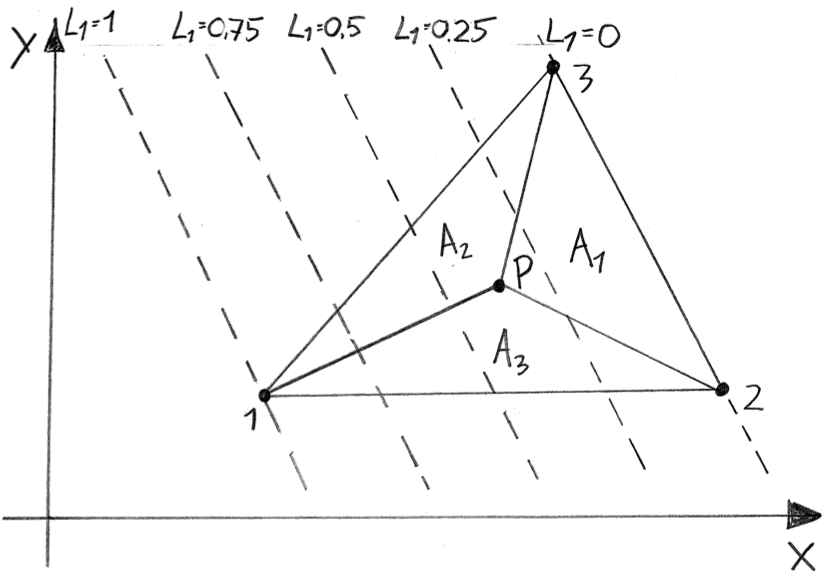
\includegraphics[width=8cm]{./images/finite_element_method_area_coords.png}
\caption{Area coordinates for a triangular element.}
\label{fig:area-coords}
\end{figure}


% upwards: rewritten from fem-engineers, p. 151-157

As with the length coordinates, the variation of area coordinates
inside an element can be illustrated, this is shown in figure
\vref{fig:graph-of-area-coords} for one element node.

% article: danish oil and natural gas, figure 3.3 page 13
\begin{figure}
  \centering
  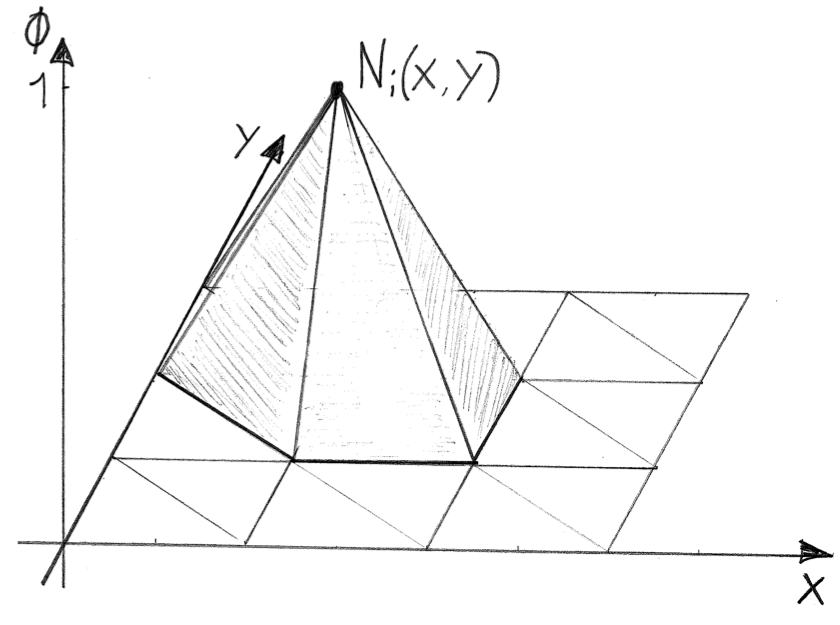
\includegraphics[width=8cm]{./images/finite_element_method_graph_of_area_coords.png}
\caption{Variation of area coordinates for one node over the entire domain.}
\label{fig:graph-of-area-coords}
\end{figure}

Note that in figure \vref{fig:graph-of-length-coords} the interpolation
functions are viewed at a particular element and that the graphs
illustrate the interpolation functions for one element. In figure
\vref{fig:graph-of-area-coords} however the interpolation functions are
viewed at one node, which means that all interpolation functions for
elements sharing this node are shown in the figure.

\subsection{Natural Coordinates in Three Dimensions}
\label{sec:natural-coordinates-3d}
We will now extend natural coordinates from two to three
dimensions for the four-node tetrahedron element.
%
% downwards rewritten from p 157-159
Natural coordinates for the four-node tetrahedron can be defined in a
manner analogous to the procedure used for the three-node triangle.

% fem-engineers figure 5.16
\begin{figure}
  \centering
  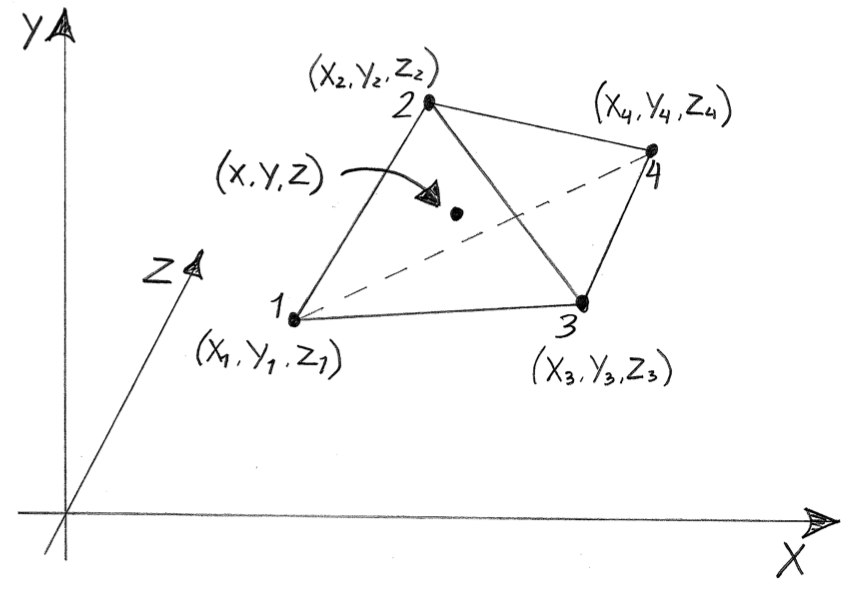
\includegraphics[width=8cm]{./images/finite_element_method_point_in_tetrahedron.png}
\caption{Tetrahedron element with global coordinates ($x$,$y$,$z$).}
\label{fig:point-in-tetrahedron}
\end{figure}

A typical four-node tetrahedron element can be see in figure
\vref{fig:point-in-tetrahedron}, the figure also defines how the nodes
are numbered. An element's global Cartesian coordinates and local
natural coordinates are related by:

\begin{equation}
\label{eq:4tetra-natural-coordinates}
\begin{aligned}
  x &= L_1 x_1 + L_2 x_2 + L_3 x_3 + L_4 x_4 \\
  y &= L_1 y_1 + L_2 y_2 + L_3 y_3 + L_4 y_4 \\
  z &= L_1 z_1 + L_2 z_2 + L_3 z_3 + L_4 z_4 \\
  1 &= L_1 + L_2 + L_3 + L_4
\end{aligned}
\end{equation}

Solving equation \eqref{eq:4tetra-natural-coordinates} gives:

\begin{equation}
\label{eq:li}
  L_i = \frac{1}{6V} ( a_i + b_i x + c_i y + d_i z), \qquad i = 1,2,3,4
\end{equation}

and

\begin{equation}
\label{eq:volume-of-tetrahedron}
6V =
\begin{array}{|cccc|}
1 & x_1 & y_1 & z_1 \\
1 & x_2 & y_2 & z_2 \\
1 & x_3 & y_3 & z_3 \\
1 & x_4 & y_4 & z_4
\end{array}
= 6 \mbox{(volume of the tetrahedron)}
\end{equation}

where examples of the constants are:

\begin{equation}
\begin{aligned}
a_1 &= 
\begin{array}{|ccc|}
x_2 & y_2 & z_2 \\
x_3 & y_3 & z_3 \\
x_4 & y_4 & z_4
\end{array}
\hspace{3mm}
c_1 = -
\begin{array}{|ccc|}
x_2 & 1 & z_2 \\
x_3 & 1 & z_3 \\
x_4 & 1 & z_4
\end{array}
\hspace{3mm}
b_1 &= -
\begin{array}{|ccc|}
1 & y_2 & z_2 \\
1 & y_3 & z_3 \\
1 & y_4 & z_4
\end{array}
\hspace{3mm}
d_1 = -
\begin{array}{|ccc|}
x_2 & y_2 & 1 \\
x_3 & y_3 & 1 \\
x_4 & y_4 & 1
\end{array}
\end{aligned}
\end{equation}

The other constants in equation \eqref{eq:li} can be obtained by
cyclic permutation of subscripts 1, 2, 3, and 4.
%
The natural coordinates for the four-node tetrahedron are also called
\defit{volumetric coordinates} and can be physically interpreted as the
ratio of volumes in a tetrahedron element. This physical
interpretation is illustrated in figure
\vref{fig:illustration-of-volume-coords}. Here the point $P$ inside the
tetrahedron divides the tetrahedron volume $V$ into four sub-volumes
$V_1$, $V_2$, $V_3$, and $V_4$. Each of these sub-volumes occupies a
part of $V$ which is equal to the coordinate ratio. Also notice
that together the sub-volumes completely covers $V$, which means that
their ratios sum to unity.

% fem-engineers figure 5.17
\begin{figure}
  \centering
  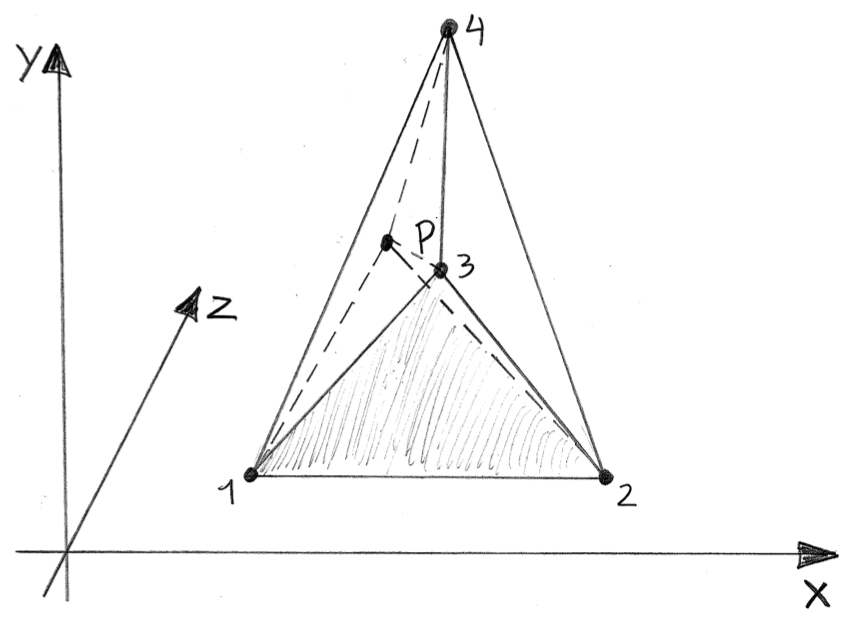
\includegraphics[width=8cm]{./images/finite_element_method_illustration_of_volume_coords.png}
\caption{Illustration of volume coordinates.}
\label{fig:illustration-of-volume-coords}
\end{figure}

We can represent the field variable $\phi$ as a function of $L_1$,
$L_2$, $L_3$, and $L_4$ (instead of $x$, $y$, and $z$) as
\citebook{page~158-159}{book:fem-engineers}:

\begin{equation}
\phi(x,y,z) = \phi_1 L_1 + \phi_2 L_2 + \phi_3 L_3 + \phi_4 L_4
\end{equation}

% upwards rewritten from p 157-159

\section{Finding the Element Properties}
\label{sec:finding-the-element-properties}
% downwards: rewritten from fem-engineers, p. 7-8
Once the elements and their interpolation functions have been
selected
%, that is: once the element model has been constructed,
we are ready to express the properties of the individual elements and
hereby determine their matrix equations.
% upwards: rewritten from fem-engineers, p. 7-8
Finding the element properties is tightly coupled with the kind of
problem we are dealing with, but in general terms the nodal values are
represented on matrix form and related by some physical laws as done in the
example in chapter \vref{sec:framework_for_equilibrium_problems} when
explaining the equilibrium
framework. The goal is to find the element stiffness matrix,
which is the stiffness matrix for a single element.
%
%Some quantities are define for each node and some for each element.
%For example nodal displacements are related to strain, where strain is
%defined for each element, and displacement for each node.

\section{Assembling the System  Equations}
\label{sec:asseble-the-element-properties}
% downwards: rewritten from fem-engineers, p. 7-8
In order to find the overall system properties, modeled by the
patchwork of elements, we must combine all the element properties
found in the previous step. In other words, the matrix equations
expressing the behavior of the elements must be combined to form the
matrix equations expressing the behavior of the entire system (the
system equations).
%The system equations have the same form as the
%equations for individual elements. The only difference being that the
%system equations contain a lot more terms because they include all
%nodes.
The assembly procedure relies on the fact that the exterior nodes
of the elements are interconnected, which means that the value of the
field variable in such a node is the same for all elements sharing the node. 
In this respect the finite element method possesses the unique feature:
The system equations are constructed by assembling the individual
element equations.
% upwards: rewritten from fem-engineers, p. 7-8
%
% downwards: rewritten from fem-engineers, p. 40
Assuming that we by some means have found the equations necessary to
describe the characteristics of the elements, then the next step
is to combine these equations. Combining the element equations
requires the same procedure regardless of the type
and complexity of problem being considered. Even if a mixture of
several different kinds of elements is used to model the system, the
procedure remains the same.
This construction procedure is, as already noted, based on the
assumption that the unknown field variable values at shared nodes are
the same for all elements connecting at that node. With this in mind
it is quite easy to combine the element equations
\citebook{page~40}{book:fem-engineers}.
% upwards: rewritten from fem-engineers, p. 40

%\subsection{Form of the System Equation}
% As the matrix equation for the full system equations for even a
% small example is very large, we will only be giving an abstract
% impression of the form of the equations. All problems generate system
% equations with the same form, as a side effect of the construction or
% the method. The stiffness matrix for system equations will always look
% like the following:

% \begin{equation}
% \label{eq:system-stiffness-matrix}
% K =
% \begin{bmatrix}
% \left[ K^{(1)} \right] & 0 & 0 & 0 \\
% 0 &\left[ K^{(2)} \right] & 0 & 0 \\
% 0 & 0 & \ddots & 0 \\
% 0 & 0 & 0 & \left[ K^{(n)} \right]
% \end{bmatrix}
% \end{equation}

% The system equations characteristics being the banded matrix. Here
% $K^{(e)}$ represent the stiffness matrix of element $e$, where $e \in
% \{1,2, ..., n\}$ and $n$ being the number of elements. The element
% stiffness matrix $K^{(e)}$, which as example could be a $4 \times 4$
% matrix, is also a banded matrix.

\subsection{The Construction Procedure}
First the dimensions of the resulting system stiffness matrix is
found. The dimensions are the same as the number of independent
variables or degrees of freedom in the system. When the dimensions are
known, then all element stiffness matrices are expanded with zero, to
have the same dimensions. The last step is to add the expanded
element stiffness matrices together. To better understand how this is
done, we show a small example.

\subsubsection{Example on Two Four-node Tetrahedron Elements}
\label{sec:example-of-two-tetrahedrons}
Consider the following example with two elements as illustrated in
figure \vref{fig:2tetra-example}.

\begin{figure}
  \centering
  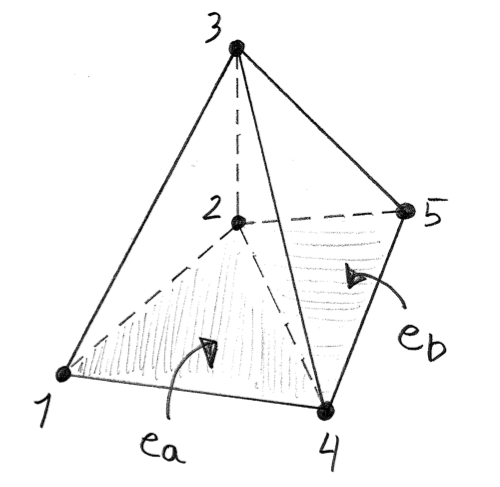
\includegraphics[width=4cm]{./images/finite_element_method_two_tetrahedrons.png}
\caption{Example of two connected four-node tetrahedra.}
\label{fig:2tetra-example}
\end{figure}

With the following element table:

\begin{table}
  \centering
\begin{tabular}{c|c|c|c|c|}
n & 1 & 2 & 3 & 4 \\
\hline
$e_a$ & 1 & 2 & 3 & 4 \\
$e_b$ & 2 & 3 & 4 & 5 \\
\hline
\end{tabular}
\caption{Element table for figure \vref{fig:2tetra-example}.}
\label{table:element-table-for-example}
\end{table}

The element stiffness matrices are:

\begin{equation}
K^a =
\begin{bmatrix}
K^a_{11} & K^a_{12} & K^a_{13} & K^a_{14} \\
K^a_{21} & K^a_{22} & K^a_{23} & K^a_{24} \\
K^a_{31} & K^a_{32} & K^a_{33} & K^a_{34} \\
K^a_{41} & K^a_{42} & K^a_{43} & K^a_{44}
\end{bmatrix}
\qquad
K^b =
\begin{bmatrix}
K^b_{11} & K^b_{12} & K^b_{13} & K^b_{14} \\
K^b_{21} & K^b_{22} & K^b_{23} & K^b_{24} \\
K^b_{31} & K^b_{32} & K^b_{33} & K^b_{34} \\
K^b_{41} & K^b_{42} & K^b_{43} & K^b_{44}
\end{bmatrix}
\end{equation}

Element $e_a$ relates forces to displacements as follows:

\begin{equation}
\label{eq:matrix-equation-for-element-a}
F^a = K^a U^a
\qquad \Leftrightarrow \qquad
\begin{bmatrix}
f^1 \\
f^2 \\
f^3 \\
f^4
\end{bmatrix}
=
\begin{bmatrix}
K^a_{11} & K^a_{12} & K^a_{13} & K^a_{14} \\
K^a_{21} & K^a_{22} & K^a_{23} & K^a_{24} \\
K^a_{31} & K^a_{32} & K^a_{33} & K^a_{34} \\
K^a_{41} & K^a_{42} & K^a_{43} & K^a_{44}
\end{bmatrix}
\begin{bmatrix}
u^1 \\
u^2 \\
u^3 \\
u^4
\end{bmatrix}
\end{equation}

And element $e_b$ like this:

\begin{equation}
F^b = K^b U^b
\qquad \Leftrightarrow \qquad
\begin{bmatrix}
f^2 \\
f^3 \\
f^4 \\
f^5
\end{bmatrix}
=
\begin{bmatrix}
K^b_{11} & K^b_{12} & K^b_{13} & K^b_{14} \\
K^b_{21} & K^b_{22} & K^b_{23} & K^b_{24} \\
K^b_{31} & K^b_{32} & K^b_{33} & K^b_{34} \\
K^b_{41} & K^b_{42} & K^b_{43} & K^b_{44}
\end{bmatrix}
\begin{bmatrix}
u^2 \\
u^3 \\
u^4 \\
u^5
\end{bmatrix}
\end{equation}

The reason for combining the system stiffness matrix this way is
directly apparent from the two element equations above. In these
equations some of the field variables are the same. The way we
combine them ensures that these field variables will not be repeated
in the final equations. \newline

The expanded element stiffness matrices are then:

\begin{equation}
K^A =
\begin{bmatrix}
K^a_{11} & K^a_{12} & K^a_{13} & K^a_{14} & 0\\
K^a_{21} & K^a_{22} & K^a_{23} & K^a_{24} & 0\\
K^a_{31} & K^a_{32} & K^a_{33} & K^a_{34} & 0\\
K^a_{41} & K^a_{42} & K^a_{43} & K^a_{44} & 0\\
0 & 0 & 0 & 0 & 0
\end{bmatrix}
\qquad
K^B =
\begin{bmatrix}
0 & 0 & 0 & 0 & 0 \\
0 & K^b_{11} & K^b_{12} & K^b_{13} & K^b_{14} \\
0 & K^b_{21} & K^b_{22} & K^b_{23} & K^b_{24} \\
0 & K^b_{31} & K^b_{32} & K^b_{33} & K^b_{34} \\
0 & K^b_{41} & K^b_{42} & K^b_{43} & K^b_{44}
\end{bmatrix}
\end{equation}

And the full system stiffness matrix:

\begin{equation}
\label{eq:system-stiffness-matrix}
K = K^A + K^B =
\begin{bmatrix}
K^a_{11} & K^a_{12} & K^a_{13} & K^a_{14} & 0\\

K^a_{21} & K^a_{22} + K^b_{11} & K^a_{23} + K^b_{12} & K^a_{24} +
K^b_{13} & K^b_{14}\\

K^a_{31} & K^a_{32} + K^b_{21} & K^a_{33} + K^b_{22} & K^a_{34} +
K^b_{23} & K^b_{24}\\

K^a_{41} & K^a_{42} + K^b_{31} & K^a_{43} + K^b_{32} & K^a_{44} +
K^b_{33} & K^b_{34}\\

0 & K^b_{41} & K^b_{42} & K^b_{43} & K^b_{44}
\end{bmatrix}
\end{equation}

The final system equations now looks like this:

\begin{equation}
F = K U
\qquad \Leftrightarrow \qquad
\begin{bmatrix}
f^1 \\
f^2 \\
f^3 \\
f^4 \\
f^5
\end{bmatrix}
= K
\begin{bmatrix}
u^1 \\
u^2 \\
u^3 \\
u^4 \\
u^5
\end{bmatrix}
\end{equation}

Note that the final system equations only include each force and
displacement once.

\section{Imposing the Boundary Conditions}
% downwards: rewritten from fem-engineers, p. 7-8
Before we can solve the system equations they must be modified to
include boundary conditions. The boundary conditions are employed to
make sure that the system in fact has a solution as discussed in
section \vref{sec:the-stiffness-matrix}.
If we have known nodal values, these are inserted, otherwise we have
to constrain parts of the system in some other way.
% upwards: rewritten from fem-engineers, p. 7-8
% more on page 48-56

\section{Solving the System Equations}
% downwards: rewritten from fem-engineers, p. 7-8
The result of the assembly procedure is a set of equations that has to be
solved simultaneously to obtain the unknown nodal values of the
problem. In a static problem a set of linear or non-linear
algebraic equations must be solved.
If instead it is a dynamic problem then the nodal unknowns
are functions of time, which generates a set of linear or non-linear
ordinary differential equations to be solved.
% upwards: rewritten from fem-engineers, p. 7-8
% more on page 56-63

\section{Making Additional Computations}
% downwards: rewritten from fem-engineers, p. 7-8
The solution found when solving the system equations is
sometimes used to calculate or find other important parameters and
values.
% upwards: rewritten from fem-engineers, p. 7-8
For example this is where we detect if and when a crack should
be propagated in our model as elaborated in section
\vref{sec:discrete-fracture-mechanics}.
